\documentclass[9pt,twocolumn,twoside]{styles/osajnl}
\usepackage{fancyvrb}
\journal{i524} 



\title{\LaTeX\ Template for Preparing an Article for I524}

\author[1,2,3]{Author One}
\author[2,*]{Author Two}
\author[1]{Author Three}

\affil[1]{Publications Department, The Optical Society (OSA), 2010 Massachusetts Avenue NW, Washington D.C., 20036}
\affil[2]{School of Science, University of Technology, 2000 J St. NW, Washington DC, 20036}
\affil[3]{School of Optics, University of Technology, 2000 J St. NW, Washington DC, 20036}

\affil[*]{Corresponding author: email@my-email.com}

\dates{\today}

\ociscodes{Cloud, I524}

%% To be edited by editor
% \doi{\url{http://gitlab.com/...}}

\begin{abstract}
This template can be used to prepare a research article for I524. Note
that this template can be run from your own \TeX\ system or within the
cloud-based \href{https://www.overleaf.com}{Overleaf} system or \href{https://www.sharelatex.com/}
{Sharelatex} systems.\newline
\end{abstract}

\setboolean{displaycopyright}{true}

\begin{document}

\maketitle

\section{Introduction}

This template is designed to assist with creating an article for I524. The page length is typically done without images. Thus if you have images in your report, please add additional content to offset the space captured by images. We do not check exactly, so there is no reason to contact us if you are a paragraph short, but if you are half a page short you may add quality content.

\section{Examples of Article Components}
\label{sec:examples}

The sections below show examples of different article components.

\section{Figures and Tables}

It is not necessary to place figures and tables at the back of the manuscript. Figures and tables should be sized as they are to appear in the final article. Do not include a separate list of figure captions and table titles.

Figures and Tables should be labelled and referenced in the standard way using the \verb|\label{}| and \verb|\ref{}| commands.

\subsection{Sample Figure}

Figure \ref{fig:false-color} shows an example figure.

\begin{figure}[htbp]
\centering
\fbox{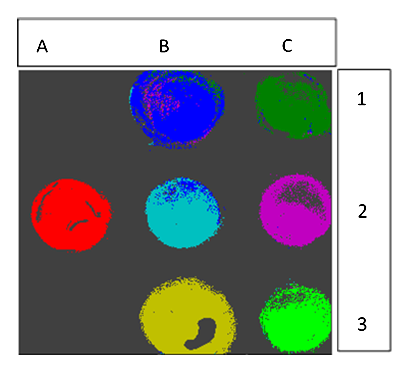
\includegraphics[width=\linewidth]{images/sample}}
\caption{False-color image, where each pixel is assigned to one of seven reference spectra.}
\label{fig:false-color}
\end{figure}

\subsection{Sample Table}

Table \ref{tab:shape-functions} shows an example table.

\begin{table}[htbp]
\centering
\caption{\bf Shape Functions for Quadratic Line Elements}
\begin{tabular}{ccc}
\hline
local node & $\{N\}_m$ & $\{\Phi_i\}_m$ $(i=x,y,z)$ \\
\hline
$m = 1$ & $L_1(2L_1-1)$ & $\Phi_{i1}$ \\
$m = 2$ & $L_2(2L_2-1)$ & $\Phi_{i2}$ \\
$m = 3$ & $L_3=4L_1L_2$ & $\Phi_{i3}$ \\
\hline
\end{tabular}
  \label{tab:shape-functions}
\end{table}

\section{Sample Equation}

Let $X_1, X_2, \ldots, X_n$ be a sequence of independent and identically distributed random variables with $\text{E}[X_i] = \mu$ and $\text{Var}[X_i] = \sigma^2 < \infty$, and let
\begin{equation}
S_n = \frac{X_1 + X_2 + \cdots + X_n}{n}
      = \frac{1}{n}\sum_{i}^{n} X_i
\label{eq:refname1}
\end{equation}
denote their mean. Then as $n$ approaches infinity, the random variables $\sqrt{n}(S_n - \mu)$ converge in distribution to a normal $\mathcal{N}(0, \sigma^2)$.

\section{Sample Algorithm}

Algorithms can be included using the commands as shown in algorithm \ref{alg:euclid}.

\begin{algorithm}
\caption{Euclid’s algorithm}\label{alg:euclid}
\begin{algorithmic}[1]
\Procedure{Euclid}{$a,b$}\Comment{The g.c.d. of a and b}
\State $r\gets a\bmod b$
\While{$r\not=0$}\Comment{We have the answer if r is 0}
\State $a\gets b$
\State $b\gets r$
\State $r\gets a\bmod b$
\EndWhile\label{euclidendwhile}
\State \textbf{return} $b$\Comment{The gcd is b}
\EndProcedure
\end{algorithmic}
\end{algorithm}

\begin{algorithm}
\caption{Python example}\label{alg:python}
\begin{quote}
\begin{Verbatim}[numbers=left]
for i in range(0,100):
  print i
\end{Verbatim}
\end{quote}
\end{algorithm}

\section{Supplemental Material}

You can include an appendix with important information and additional figures if needed. HOwever they must be referenced and follow the same guidelines as in the main text.
All materials must be associated with a figure, table, or equation or be referenced in the results section of the manuscript. 
(1) 2D and 3D image files and video must be labeled “Visualization,” not “Movie,” “Video,” “Figure,” etc. 
(2) Machine-readable data (for example, csv files) must be labeled  “Data File.”  Number data files and visualizations consecutively, e.g., “Visualization 1, Visualization 2….”
(3) Large datasets or code files must be placed in an open, archival database.  Such items should be mentioned in the text as either “Dataset” or “Code,” as appropriate, and also be cited in the references list.  For example, “see Dataset 1 (Ref. [1]) and Code 1 (Ref [2]).” Here are examples of the references: 

\subsection{Sample Dataset Citation}

1. M. Partridge, "Spectra evolution during coating," figshare (2014) [retrieved 13 May 2015], http://dx.doi.org/10.6084/m9.figshare.1004612.

\subsection{Sample Code Citation}

2. C. Rivers, "Epipy: Python tools for epidemiology" (Figshare, 2014) [retrieved 13 May 2015], http://dx.doi.org/10.6084/m9.figshare.1005064.

\section{Funding Information}

Funding information should be listed in a separate block preceding any acknowledgments. List just the funding agencies and any associated grants or project numbers, as shown in the example below:

National Science Foundation (NSF) (1263236, 0968895, 1102301); The 863 Program (2013AA014402).

The acknowledgments may contain any information that is not related to funding:

The authors thank H. Haase, C. Wiede, and J. Gabler for technical support.

Do not use Funding Information or Acknowledgment headings.

\section{References}

The best programs to manage your references is jabref or emacs. You can edit the references and verify them with them for format errors. To cite them use the citation key. You can add multiple bib files to the bibliography command separated by comma.

\bigskip
\noindent Add citations with the cite command. See \cite{Zhang:14,OSA,FORSTER2007}.

% Bibliography
\bibliography{references}

% Full bibliography added automatically for Optics Letters submissions; the following line will simply be ignored if submitting to other journals.
% Note that this extra page will not count against page length
\bibliographyfullrefs{references}
 
%Manual citation list
%\begin{thebibliography}{1}
%\bibitem{Zhang:14}
%Y.~Zhang, S.~Qiao, L.~Sun, Q.~W. Shi, W.~Huang, %L.~Li, and Z.~Yang,
 % \enquote{Photoinduced active terahertz metamaterials with nanostructured
  %vanadium dioxide film deposited by sol-gel method,} Opt. Express \textbf{22},
  %11070--11078 (2014).
%\end{thebibliography}

% Please include bios and photos of all authors for aop articles 
\ifthenelse{\equal{\journalref}{aop}}{%
\section*{Author Biographies}
\begingroup
\setlength\intextsep{0pt}
\begin{minipage}[t][6.3cm][t]{1.0\textwidth} % Adjust height [6.3cm] as required for separation of bio photos.
  \begin{wrapfigure}{L}{0.25\textwidth}
    
\includegraphics[width=0.25\textwidth]{images/john_smith.eps}
  \end{wrapfigure}
  \noindent
  {\bfseries John Smith} received his BSc (Mathematics) in 2000 from The University of Maryland. His research interests include lasers and optics.
\end{minipage}
\begin{minipage}{1.0\textwidth}
  \begin{wrapfigure}{L}{0.25\textwidth}
    
\includegraphics[width=0.25\textwidth]{images/alice_smith.eps}
  \end{wrapfigure}
  \noindent
  {\bfseries Alice Smith} also received her BSc (Mathematics) in 2000 from The University of Maryland. Her research interests also include lasers and optics.
\end{minipage}
\endgroup
}{}


\end{document}
